\chapter{INTRODUCTION\label{chapter:introduction}}


The ever-increasing proliferation of online text means that information is available on essentially any topic, but it also becomes increasingly difficult to find as more and more irrelevant information needs to be sifted through.  
As of the writing of this, the internet is estimated to have 1.2 billion websites \citep{internetstats}.  To give a richer picture, English Wikipedia has about 5.5 million pages with more than 700 new articles being added each day \citep{wiki:wikistats}.  The popular open-access scientific e-print service, arXiv\footnote{\url{https://arxiv.org/}} now has almost 1.3 million articles and receives over 10,000 new article submissions each month \citep{arXivstats}, and the open-access biomedical database PubMed\footnote{\url[https://www.ncbi.nlm.nih.gov/pubmed]} contains well over 27 million articles.  

Clearly, ever-improving tools are needed to handle this massive (and growing) abundance of information, and as the vast majority of this data is in the form of natural language (rather than a structured database), these tools must operate over natural language queries and natural language results.  While certain queries and results can be anticipated using statistics, in order to handle a new query, the system must be able to \emph{infer} what the desired result is from the query.  
While this natural language inference is at the heart of several natural language processing (NLP) tasks, it is particularly crucial for the task of question answering. 
%This natural language inference is critical to search as well as many other types of natural language processing tasks including question answering.  


\begin{figure}[t!]
\centering
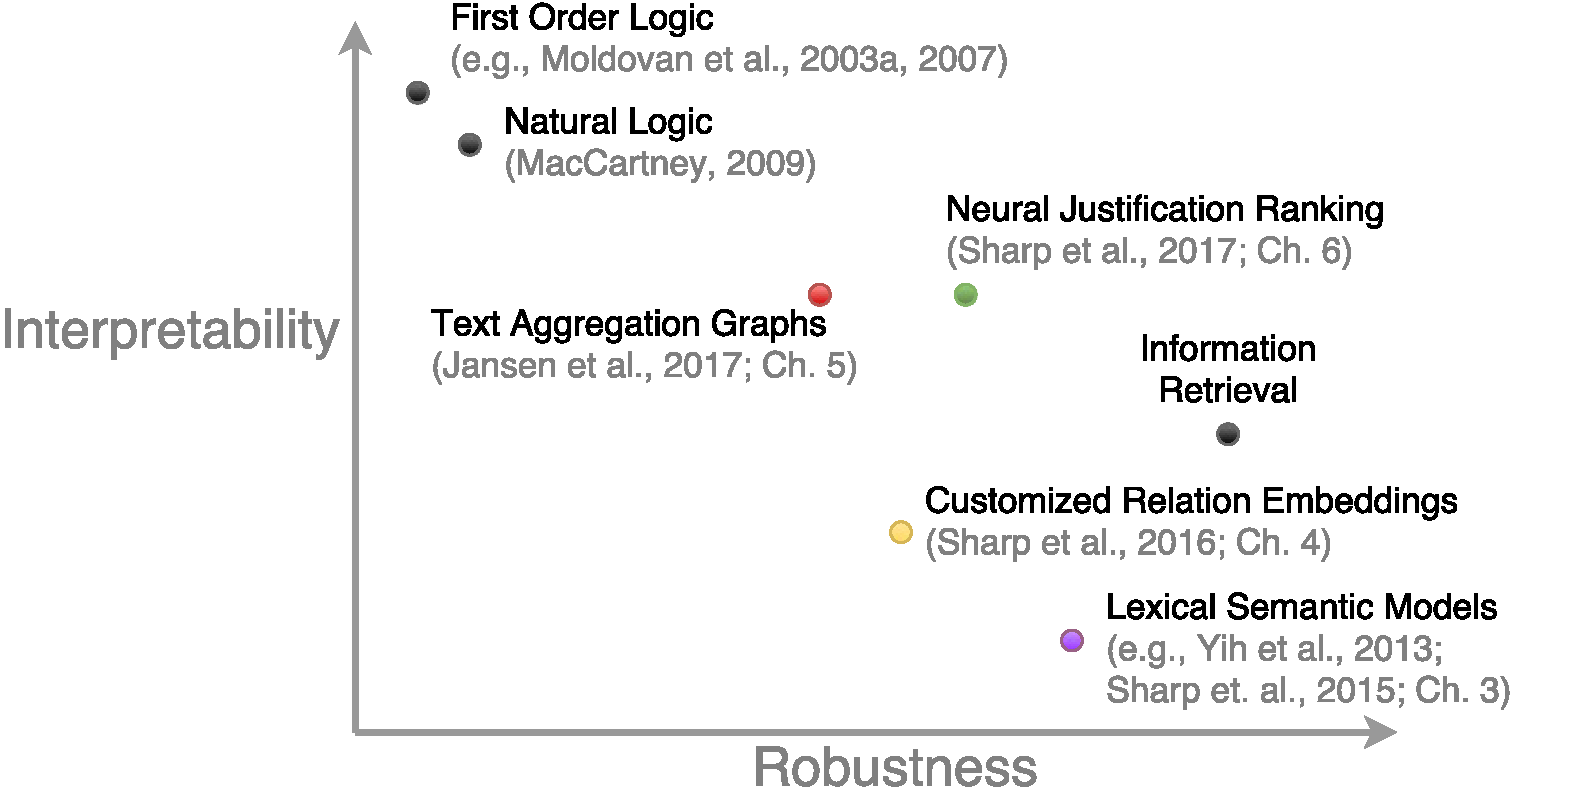
\includegraphics[width=1.0\textwidth]{mainmatter/continuum_new.pdf}
\caption{In this work we focus on two desirable aspects of a question answering approach: robustness and interpretability.  Here we plot several approaches, including the four that are the focus of this work (the colored dots, please see corresponding chapters for model details), in terms of these aspects.  Note that the ideal model would be found in the upper right-hand corner -- robust to language variation and easily interpretable by a human user.}
\label{fig:continuum}
\end{figure}

Question answering (QA), i.e., finding short answers to natural language questions, is one of the most important but challenging 
tasks on the road towards natural language understanding~\citep{Etzioni:11}. 
%\address{Require bridging lexical chasm}
As mentioned above, a QA system first faces the challenge that both the question and any potential answer sources are in the form of natural language, which inherently contains a large degree of lexical, syntactic, and even dialectal variation.
Additionally, unlike search or information retrieval, answers often don't contain lexical overlap with the question (e.g. {\em What should we eat for breakfast? -- Zoe's Diner has good pancakes}).  This requires QA models to draw upon more complex methods to bridge this "lexical chasm" \citep{Berger:00}, i.e., to infer what the answer should be.  These methods range from robust shallow models based on lexical semantics (e.g., the model of \citet{yih13} which is based on semantic relations such as \textit{hypernymy} and \textit{synonymy} as well as distributional similarity), to deeper, explainably-correct, but much more brittle inference methods based on first order logic (e.g., the Natural Logic of \citet{maccartney2009natural} that uses hand-crafted logic rules that operate over natural language).  We exemplify this continuum in Figure \ref{fig:continuum}, which relates examples of previous approaches (described in Chapter \ref{chapter:related_work}) to our four approaches (see Chapters \ref{chapter:naacl2015} through \ref{chapter:emnlp2017}) in terms of their robustness (Section \ref{sec:robustness}) and their interpretability (Section \ref{sec:interpretability}).  

%Lexical semantic approaches, such as the model of \citet{yih13} which is based on semantic relations between words (such as \textit{hypernymy} and \textit{synonymy}) and distributional similarity\footnote{Distributional similarity is essentially defining a word by its lexical context (i.e., its \textit{distribution}.}, are robust but shallow -- they can score any answer, but they struggle to operate over larger, multi-word contexts (e.g., \textit{stick} versus \textit{stick shift}) or word sense disambiguation (e.g., the difference between a \textit{computer mouse} and the animal).  Their interpretability is also typically quite low, as they are able only to provide a set of association scores for the words in the question and answer, which is difficult for a human user to interpret.
%On the other end of the spectrum are formal approaches which attempt to prove answers by using sets of hand-crafted semantic rules to reason over formal representations (e.g., \citep{moldovan2003cogex,moldovan2007cogex}) or over natural language (e.g., the Natural Logic of \citet{maccartney2009natural}).  While these approaches are very interpretable when they succeed (they result in a formally valid proof), they fail whenever the content of the question or answer is not covered by the existing set of rules -- a frequent occurrence, given the variation that exists in natural language.  

%\address{Natural language inference (NLI)}
\section{Robustness}
\label{sec:robustness}

While first order logic methods are attractive for their formality, it is this same formality that renders them too brittle to be of much use outside of small, toy domains.  In order to be used, these methods require parsing natural language into formal meaning representations (a task which is very difficult given the previously mentioned language variations) and then performing inference over these representations using logic rules and axioms, again made more difficult by the open-domain (i.e., questions can be about anything and of any level of complexity) and the fact that there are never enough rules and axioms to encode everything you need to know about the world and language.  Here we focus on \emph{approximating} this formal logic inference using natural language and machine learning instead of formal representations and hand-crafted rules.  While we lose some of the ability to \emph{prove} an answer, we gain much-needed robustness to both language and domain.

Many of these shallower methods that are based on machine learning  (rather than pre-written rules) require a large amount of supervised training data, that is, data for which the label is known.  In the context of QA, these are questions for which we know the \emph{true} answer(s)\footnote{The true, or gold, answer to a question can be debatable, and there are many situations in which there can be more than one correct answer.  Typically, an answer is considered correct if a human expert labels it as such, but again, this is open to interpretation.}. In many domains, however, this requirement is expensive as it \rev{is difficult to find large amounts of high-quality data (i.e., complete explanations and little irrelevant information)}.  Therefore, in this work, we emphasize methods which use semi- and distant supervision\footnote{With semi-supervision, you begin with a small amount of hand-labeled data and learn to label new examples automatically, expanding your pool of labeled examples.  With distant supervision, the labeling is done automatically from the start, e.g., by aligning a database of known facts with free text instances containing portions of those facts.  For example, if you have a fact triple such as \textit{(Jane\_Smith, president\_of, College\_X)}, you can find all sentences that contain those three elements and count them all as correct instances of the relation \textit{president\_of}.  This type of approach is able to scale to large data-sources, but is very prone to noise (e.g., not all sentences truly demonstrate the \textit{president\_of} relation).}, rather than needing a large amount of hand-generated training data.  This emphasis allows these methods to be applicable across a wider variety of domains.   

Another potential problem associated with these shallower, machine learning-based methods is that with the relaxation of the formality, the explainability may also be lost, and with it the ability to understand \emph{why} the model produces the answers it does.  
Without this understanding, users cannot easily discern sources of error or determine how to fix them (which is critical for industry applications, where users are typically not NLP experts).  Additionally, if a model cannot explain why it makes the predictions it does, it does not allow a user to trust the prediction, which becomes more important in high-stakes scenarios, such as in medical or military applications. 
%This model understanding is critical for being able to discern sources of model errors and fix them to attain better performance or generalization. 
%\address{why we care about explainability}
To address interpretability, we include models (Chapters \ref{chapter:cl2017} and \ref{chapter:emnlp2017}, see also Section \ref{sec:interpretability}) that use a human-readable intermediate output generated by the model from background knowledge to provide an explanation for the inference performed by the model.  \rev{This answer justification can be thought of as proxy for a formal proof, where the background knowledge serves as an approximation for the axioms and the method by which we form the justification serves approximates the inference rules.  In our approaches, which only approximate formal inference rather than abiding by the rigid structure of first order logic, however, we gain the robustness of a statistical approach. }

%\address{We try/test our NLI methods in the domain of Question answering (QA):}

% \address{QA hard bc of}

% emnlp2016 intro
%Question answering (QA), i.e., finding short answers to natural language questions, is one of the most important but challenging tasks on the road towards natural language understanding~\cite{Etzioni:11}. 
%\address{Require bridging lexical chasm}
%Unlike search or information retrieval, answers infrequently contain lexical overlap with the question (e.g. {\em What should we eat for breakfast? -- Zoe's Diner has good pancakes}), and require QA models to draw upon more complex methods to bridge this "lexical chasm" \cite{Berger:00}.  These methods range from robust shallow models based on lexical semantics, to deeper, explainably-correct, but much more brittle inference methods based on first order logic.  

%\address{One approach to bridging lexical chasm is use of monolingual alignment models, but: }

\subsection{Aligning questions and answers}
\label{sec:intro_naacl2015}
%\address{these are expensive to train (need lots of gold QA pairs)}
% naacl2015 intro
\citet{Berger:00} proposed that the "lexical chasm", or lack of lexical overlap that often exists between questions and answers, might be partially bridged by making use of techniques popular in machine translation, the task of automatically translating text from one language to another language.  At a high level, in typical machine translation, a model is given a sentence in one language aligned with its translation in another language.  The model keeps track of statistics such as how frequently words in each language co-occur in the sentence-translation pairs and uses these statistics to generate word-alignment scores.  \citeauthor{Berger:00} suggested repurposing these statistical machine translation models for QA. Instead of translating text from one language to another, these \emph{monolingual} alignment models (i.e., models that align words within the same language) learn to translate from question to answer\footnote{In practice, alignment for QA is often done from answer to question, as answers tend to be longer and provide more opportunity for association~\citep{Surdeanu:11}.}.  Given the previously mentioned example question, {\em What should we eat for breakfast? -- Zoe's Diner has good pancakes}, these models learn common associations from question terms such as {\em eat} or {\em breakfast} to answer terms like {\em kitchen, pancakes, or cereal}, and the strength of the association serves as a proxy for the validity of the inference.

\begin{table}[t]
\begin{center}
\begin{tabularx}{0.8\linewidth}{p{1.5cm}p{10cm}}
%\multicolumn{2}{p{15cm}}{\textbf{High quality} Which of these is a response to an internal stimulus?} \\
\hline 
 Quality & Question and Community-Chosen Answer \\
 \hline
 High & Q: What causes a cat to lose its fur? \\
 		& A: It could be a dietary issue, such as an allergy, or a more serious physical condition...\\
 	&	\\
 Fair &  Q: What causes you to fart alot? \\
 		&	A: Broccoli	\\
 &		\\
 Poor	&	Q: What causes sheets to get little balls on them. I think it is called pilling? \\
 		 &  A: i've always wondered the same thing \\
\end{tabularx}
\caption{{  Examples of questions from Yahoo! Answers, a community question answering website, demonstrating the variable quality of the community-chosen \textit{best} answer. }}
\label{tab:cqa_quality}
\end{center}
\end{table}

While monolingual alignment models have enjoyed a good deal of recent success in QA (see Section \ref{sec:related_work_naacl2015} for more discussion), they have expensive training data requirements,  
requiring a large set of aligned in-domain question-answer pairs for training.
In most domains these pairs are expensive to generate, and one of the current methodological challenges in QA is locating or building QA pairs \rev{that are high enough quality (in terms of answer completeness, question variety, and topic coverage) to be used for training and testing}. Even large open-domain international evaluations and workshops such as the Text REtrieval Conference (TREC)\footnote{\url{http://trec.nist.gov}} and the Cross Language Evaluation Forum (CLEF),\footnote{\url{http://www.clef-initiative.eu}} are often limited to sets of a few hundred factoid questions, many of which are highly related.  As a result, for open domain QA one often makes use of Community Question Answering data from websites such as Yahoo! Answers or Stack Overflow, which offer tens of thousands of questions, but of highly variable quality, as demonstrated with the example questions in Table \ref{tab:cqa_quality}.  
\rev{While techniques have been developed to automatically generate new questions using syntactic rearranging, templates and fact databases, or deep neural networks \citep[e.g.,][]{Heilman2010GQS, Serban2016GeneratingFQ, du2017question}, at the current state of the art they often create questions and answers that are overly simplistic, repetitive, and unlike natural language (often not even syntactically valid).  Additionally, the neural network based methods for generation also often have heavy training requirements themselves.}
For low-resource languages or specialized domains like science or biology, often the only option is to enlist a domain expert to generate gold QA pairs --  a process that is both expensive and time consuming.  All of this means that only in rare cases are we accorded the luxury of having enough QA pairs to properly train an alignment model, and so these models are often underutilized or left struggling for resources. 

%\address{We propose a method for generating artificial training data (can be thought of as a form of distant supervision?? If you squint?) (NAACL2015)}
% naacl2015 intro
Making use of recent advancements in discourse parsing \citep{feng12}\footnote{Discourse parsing involves the segmentation of text into adjacent spans which are then recursively joined and assigned both a direction (which span is the head, and which is the dependent) and a label (e.g., \emph{elaboration}, \emph{contrast}, \emph{attribution}, etc).},  
in Chapter \ref{chapter:naacl2015} we address this issue, and investigate whether alignment models for QA can be trained from \emph{artificial} question-answer pairs generated from discourse structures  imposed on free text.  Specifically, we align the words from the head and the dependent of each discourse relation in lieu of a question and answer.  That is, given a sentence such as \textit{Water is an efficient solvent because of this polarity}, which has the discourse relation [\textit{Water is an efficient solvent}] $\rightarrow_{cause}$ [\textit{because of this polarity}], we learn alignments between words from the discourse relation's head (e.g., \textit{water} and \textit{solvent}) and its dependent (e.g., \textit{polarity}).
This method can be thought of as a form of distant supervision, as we don't have true labels for which free-text pairs are truly adequate proxies for question-answer pairs.
% by imposing structure on inexpensive free text resources instead of using QA pairs.  
We evaluate our methods on two corpora, generating alignment models for an open-domain community QA task using Gigaword\footnote{LDC catalog number LDC2012T21}, and for a biology-domain QA task using a biology textbook. 


\subsection{Customizing approaches to a specific question type}
\label{sec:intro_emnlp2016}
%\address{Diff info needs and so the “manner” by which the lexical chasm is bridged should hopefully be robust to that}

This alignment approach for QA can be considered as falling into a larger group of approaches which prefer answers that are closely related to the question, where the relatedness is determined by the associations of the alignment model (e.g., as briefly referred to in Section \ref{sec:intro_naacl2015}) or by associations provided by other lexical semantic models such as word embeddings~\citep{yih13,jansen14,fried2015higher}. 
While appealing for its robustness to natural language variation, this one-size-fits-all category of approaches does not take into account the wide range of distinct question types that can appear in any given question set (see, e.g.,  Table \ref{tab:inferenceexamples}), and that are best addressed individually~\citep{chu2004ibm,ferrucci2010building,clark2013study} for a specific question set.  

%These don’t address diff types of inference/info needs:
%\address{We propose a framework for learning customized alignments/associations for a specific info need using semi-supervised methods (EMNLP2016)}
Given the variety of question types, we suggest that a better approach is to look for answers that are related to the question \emph{through the appropriate relation}, e.g., a causal question, should have a cause-effect relation with its answer.  For example, to score a candidate answer for a question such as \emph{What do hurricanes cause?}, while general purpose word associations would give a high score to a sentences containing near associates such as \emph{tornadoes} and \emph{tropical storms}, we suggest that a better approach would be using a set of relation-specific word associations that would provide high scores for words that are in a cause-effect relation with \emph{hurricane}, such as \emph{flooding} or \emph{damage}.
Adopting this view, and working with embeddings as a mechanism for assessing relationship, in Chapter \ref{chapter:emnlp2016} we address a key question: how do we train and use task-specific embeddings cost-effectively? 
Using causality as a use case, we answer this question with a framework for producing causal word embeddings, i.e., a set of word embeddings which encode causality rather than similarity, with minimal supervision, and a demonstration that such task-specific embeddings significantly benefit causal QA. 

\section{Interpretability}
\label{sec:interpretability}

%\address{BUT, these shallower methods lose some of the explainability (get only a set of associations and weights on association features), so we develop approaches that focus on explanation, aggregation, and robustness}

%\address{two approaches (one more structured, one with learned representations) for answering science questions and providing compelling, human-readable explanations for the answers.}

%\address{Latent layer/intermediate output learned during training which correlates with what the model is learning}

% ------ pasted from emnlp2017-------------
%\todo{I don't think this text really fits here at all - perhaps move back to the paper/chapter intro and write something else for here}

Developing interpretable machine learning models, that is, models where a human user can \emph{understand} what the model is learning, is considered by many to be crucial for ensuring usability and accelerating progress \citep{craven1996extracting,Kim2015MindTG, letham2015interpretable, Ribeiro2016WhySI}.  
% bs: removed for space, we talk more about this in related work
%As such, it has received much attention in recent years, especially as deep learning and complex architectures have seen dramatic gains in many tasks.
For many applications of question answering (QA), simply providing an answer (or even an answer alongside a list of word-associations and their corresponding model weights, as with the approaches briefly described in Section \ref{sec:robustness}) is not sufficient. 
\rev{For example, in the medical domain, a user would not trust a system that recommends invasive procedures without giving a justification as to why (e.g., ``Smith (2005) found procedure \emph{X} healed 90\% of patients with heart disease who also had secondary pulmonary complications'').  Additionally, a QA tool is more useful when its human user can identify both when it functions correctly, and when it delivers an incorrect or misleading result -- especially in situations where incorrect results carry a high cost.  
For this reason we include methods that are interpretable, i.e., able to {\em explain} why an answer is correct.}

One approach to interpreting complex models is to make use of human-interpretable information generated by the model to gain insight into what the model is learning.  
We follow the intuition of \citet{Lei2016RationalizingNP}, whose two-component network first generates text spans from an input document, and then uses these text spans to make predictions.   \citeauthor{Lei2016RationalizingNP} utilize these intermediate text spans to infer the model's preferences.
By learning these intermediate representations end-to-end with a downstream task (i.e., question answering or another task that the user is interested in), they are optimized to correlate with what the model learns is discriminatory for the task, and they can be evaluated against what a human would consider to be important.  

\subsection{Multiple choice science questions as a proving ground}
\label{sec:mcqa}

\begin{table}[t]
\begin{center}
\begin{tabularx}{\linewidth}{p{1cm}p{13cm}}
\multicolumn{2}{p{15cm}}{\textbf{Question:} Which of these is a response to an internal stimulus?} \\
 (A) & A sunflower turns to face the rising sun. \\
 (B) & A cucumber tendril wraps around a wire. \\
 (C) &  A pine tree knocked sideways in a landslide grows upward in a bend. \\
 (\textbf{D}) &\textbf{Guard cells of a tomato plant leaf close when there is little water in the roots .} \\
\\
\multicolumn{2}{p{15cm}}{\textbf{Justification:} 
Plants rely on hormones to send signals within the plant in order to respond to internal stimuli such as a lack of water or nutrients. } \\
\end{tabularx}

\caption{{  Example of an 8th grade science question with a justification for the correct answer that completes the needed inference between question and answer.  Note the lack of direct lexical overlap present between the justification and the correct answer, demonstrating the difficulty of the task of finding justifications using traditional distant supervision methods. }}

\label{tab:question_example}
\end{center}
\end{table}

\begin{table*}[t]
\begin{center}
\small
\begin{tabularx}{\textwidth}{p{2.5cm}p{5.2cm}p{5.9cm}}
\hline
Category &	\multicolumn{2}{l}{Example} \\
\hline
Retrieval	&	\multicolumn{2}{l}{Q: The movement of soil by wind or water is called:} \\
(35\%)		&   (A) condensation   	&	(B) evaporation   \\
			&	(C) erosion   		&	(D) friction \\
\\
General 	&	\multicolumn{2}{l}{Q: Which example describes an organism taking in nutrients?} \\
Inference	&   (A) A dog burying a bone			&   (B) A girl eating an apple	\\
(39\%)		&	(C) An insect crawling on a leaf	&  (D) A boy planting tomatoes in the garden  \\
\\
Model-based & 	\multicolumn{2}{l}{Q: When a baby shakes a rattle, it makes a noise. Which form of} \\
Inference	& 	\multicolumn{2}{l}{energy was changed to sound energy?} \\
(26\%)		&	(A) electrical	&   (B) light   \\
			&	(C) mechanical	&   (D) heat  \\
			
\end{tabularx}
\caption{ 
Categories of questions and their relative frequencies as identified by \citet{clark:2013}. Retrieval-based questions (including \emph{is--a}, dictionary definition, and property identification questions) tend to be answerable using information retrieval methods over structured knowledge bases, including taxonomies and dictionaries. 
More complex general inference questions make use of either simple inference rules that apply to a particular situation, a knowledge of causality, or a knowledge of simple processes (such as \emph{solids melt when heated}).
Difficult model-based reasoning questions require a domain-specific model of how a process works, like how gravity causes planets to orbit stars, in order to be correctly answered.
Note here that we do not include diagram questions, as they require specialized spatial reasoning that is beyond the scope of this work. }
\label{tab:inferenceexamples}
\end{center}
\end{table*}

In Chapters \ref{chapter:cl2017} and \ref{chapter:emnlp2017}, we apply this general framework for model interpretability to QA, and in particular to answering multiple-choice science exam questions \citep{clark:2015}, by generating a human-readable justification for each selected answer.  An example science exam question is provided in Table~\ref{tab:question_example} to demonstrate the role of the justification in explaining the correct answer choice as well as to illustrate the fact that retrieving such a justification is non-trivial due to lack of lexical overlap. 
%Science exams are an important proving ground for QA because inference is often required to arrive at a correct answer, and, commonly, incorrect answers that are high semantic associates of either the question or correct answer are included to ``lure'' students (or automated methods) away from the correct response.

In addition to the general difficulties of QA previously described, this particular QA domain is challenging as approximately 70\% of science exam questions have been shown to require complex forms of inference to solve \citep{clark:2013,jansen-EtAl:2016:COLING} \rev{(and indeed, we also have difficulty with this, see Sections \ref{sec-cl2017:erroranalysis} and \ref{sec-emnlp2017:erroranalysis})}.  In Table \ref{tab:inferenceexamples} we provide example questions from each of the three main categories of questions from \citet{clark:2013}, where the categories are based on the methods likely required to answer them correctly.  Not only do the majority of questions require some form of inference to solve (i.e., there is little or no lexical overlap between question and answer), but there are few structured knowledge bases to support this inference, and also commonly incorrect answers that are high semantic associates of either the question or correct answer are included to ``lure'' students (or automated methods) away from the correct response.

\rev{Having answer choices at all, however, no matter how closely related, does make this task simpler than if we were given the same questions with no answer options (open-ended QA).  With open-ended QA, the system first needs to find a large pool of candidate answer texts, with no guarantee that the correct answer is there.  Additionally, while multiple-choice questions are straightforward to evaluate, a correct answer to an open-ended question may be expressed in a variety of ways, making automatic evaluation problematic. We do not explore these challenges here, as we instead isolate the task of learning approximate inference from a question to a given answer, but our approaches could be extended to include the candidate answer generation and evaluation components needed for open-ended QA. }

\subsection{Reranking justifications with weak supervision}
\label{sec:reranking_justifications}

Within the domain of multiple-choice science QA, we propose two approaches that reframe QA from the task of scoring (or reranking) answers to a process of \emph{generating and evaluating justifications} for why a particular answer candidate is correct.  
Each of these approaches learn to both select and explain answers, when the only supervision available is for which answer is correct (but not how to explain it).
Intuitively, our approaches choose the justifications that provide the most help towards ranking the correct answers higher than incorrect ones.  
More formally, our approaches alternate between using the current model to choose the highest scoring justifications for answers, and optimizing the answer ranking model given these justifications. 
Thus, for both of these approaches, for each question and candidate answer we gather (or create) a pool of potential justifications.  Then we allow the model to learn how to rerank these justifications such that the highest-scoring justification for the correct answer is better than the highest-scoring justification for any of the incorrect answers.   
Crucially, for both approaches, these reranked texts serve as our human-readable answer justifications, and by examining them, we gain insight into what the model learned was useful for the QA task. 

The first approach (Chapter \ref{chapter:cl2017}) uses aggregation of information from several sources along with structured representations of the text to create justifications of the answer choices.  
In particular, we aggregate multiple sentences into hierarchical graph structures (called text aggregation graphs, Section \ref{sec-cl2017:tag}) that capture both intrasentence syntactic structures and intersentence lexical overlaps. 
Further, we model whether the intersentence lexical overlap is between contextually relevant keywords critical to the justification, or other words which may or may not be relevant. These justifications provide the inference needed to answer the question.

The second (Chapter \ref{chapter:emnlp2017}) uses a shallower approach without aggregation or structured representations.  In this shallow approach, we consider only justifications which are single sentences from a corpus and we replace the graph representation of sentences with embeddings and a small set of explicit features (that model lexical overlap, length, etc).  These changes allow us to operate over larger text resources.  

Despite the differences between these two approaches, however, each allows us to address the challenge of question answering while prioritizing interpretability of the model.

%------end paste from emnlp 2017--------------------------


%\address{Applied to science MCQA }

%\address{Description (clark and jansen stuff)}

%\address{Lure answers}

%To encourage a emphasis on the task of explainable inference for question answering (QA), \citet{clark:2015} introduced the Aristo challenge, a QA task focused on developing methods of automated inference capable of passing standardized elementary school science exams, while also providing human-readable explanations (or justifications) for those answers.  Science exams are an important proving ground for QA because inference is often required to arrive at a correct answer, and, commonly, incorrect answers that are high semantic associates of either the question or correct answer are included to ``lure'' students (or automated methods) away from the correct response.
%
%  In spite of being multiple choice, these questions tend to be  more challenging than factoid QA, which is highly amenable to retrieval-based models that operate over large structured knowledge bases such as Freebase (e.g. \note{Liang?, etc}). \todo{The previous sentence must be defended.} Multiple choice exams also commonly contain "lure" answers -- incorrect answers that are high semantic associates of either the question or correct answer -- which further reduce the efficacy of retrieval or lexical semantic/associative methods. 
%- Semantic Parsing for QA / Freebase (Percy Liang), much easier problem
%
%-- Science exams as a challenging QA problem
%- More than just factoid lookup, despite being multiple choice
%- Interesting proving ground for QA -- questions are challenging, and well-constructed multiple-choice questions typically have lure answers that are incorrect but are highly associated with either the question or correct answer, making shallow methods difficult (REF). 
%

%Adding to the challenge, not only is inference required for science exams, but several kinds of inference are present.
%In an analysis of three years of standardized science exams, \citet{clark:2013} identified three main categories of questions based on the methods likely required to answer them correctly. Examples of these questions can be seen in Table~\ref{tab:inferenceexamples}, highlighting that 65\% of questions require some form of inference to be answered.
%
%\begin{table*}[t]
%\caption{ 
%Categories of questions and their relative frequencies as identified by \citet{clark:2013}. Retrieval-based questions (including \emph{is--a}, dictionary definition, and property identification questions) tend to be answerable using information retrieval methods over structured knowledge bases, including taxonomies and dictionaries. 
%More complex general inference questions make use of either simple inference rules that apply to a particular situation, a knowledge of causality, or a knowledge of simple processes (such as \emph{solids melt when heated}).
%Difficult model-based reasoning questions require a domain-specific model of how a process works, like how gravity causes planets to orbit stars, in order to be correctly answered.
%Note here that we do not include diagram questions, as they require specialized spatial reasoning that is beyond the scope of this work. 
%}
%\begin{center}
%\small
%\begin{tabularx}{\textwidth}{p{2cm}p{5cm}p{5.9cm}}
%\hline
%Category &	\multicolumn{2}{l}{Example} \\
%\hline
%Retrieval	&	\multicolumn{2}{l}{Q: The movement of soil by wind or water is called:} \\
%(35\%)		&   (A) condensation   	&	(B) evaporation   \\
%			&	(C) erosion   		&	(D) friction \\
%\\
%General 	&	\multicolumn{2}{l}{Q: Which example describes an organism taking in nutrients?} \\
%Inference	&   (A) A dog burying a bone			&   (B) A girl eating an apple	\\
%(39\%)		&	(C) An insect crawling on a leaf	&  (D) A boy planting tomatoes in the garden  \\
%\\
%Model-based & 	\multicolumn{2}{l}{Q: When a baby shakes a rattle, it makes a noise. Which form of energy was} \\
%Inference	& 	\multicolumn{2}{l}{changed to sound energy?} \\
%(26\%)		&	(A) electrical	&   (B) light   \\
%			&	(C) mechanical	&   (D) heat  \\
%			
%\end{tabularx}
%\label{tab:inferenceexamples}
%\end{center}
%\end{table*}
%
%
%%-- Approximate Inference/Continuum
%%- benefits/drawbacks
%%- Alignment/Lexical semantic end: Robust but lacks justifications
%%- First-order Logic end: Brittle, but provably correct justifications
%%- Meeting in the middle (relax FOL, or impose more structure into LS)
%
%
%%-- Justifications as central to question answering
%%- In many applications, answering without justifications is pointless
%%- Example (medical -- you need surgery, but not explain why)
%%- Model QA as generating and evaluating explanations/justifications for why a particular answer candidate is correct
%
%
%
%%-- Reframing QA as a generating and evaluating explanations/justifications for why a particular answer candidate is correct
%
%To address these issues, here we reframe QA from the task of scoring (or reranking) answers to 
%a process of \emph{generating and evaluating justifications} for why a particular answer candidate is correct. 
%We focus on answering science exam questions, where many questions require complex inference, and building and evaluating answer justifications is challenging. 

%\address{To get a complete and valid explanation for selection of answer choice, may need to aggregate info from multiple distinct resources}

%\address{For aggregation, to prevent semantic drift, use structured representations (parts of CL2017)}
%In particular, we construct justifications by {\em aggregating} multiple sentences from a number of textual knowledge bases (e.g., study guides, science dictionaries), which, in combination, aim to explain the answer.
%We then rank these candidate justifications based on a number of measures designed to assess how well integrated, relevant, and on-topic a given justification is, and select the answer that corresponds to the highest-ranked justification.

%\address{Robustness - shallower, no structure, learned representations (EMNLP2017-hopeful)}


% ----------CONTRIBUTIONS-
\section{Contributions}
\label{sec:Contributions}

With this work we tackle the challenging task of question answering, seeking methods which balance the (sometimes conflicting) demands of robustness and interpretability.  We  address these challenges with four approaches.  In particular, the specific contributions of this work are:


% naacl 2015
\subsection{Contribution 1: Using discourse structures to generate artificially aligned pairs for training question answering models} 
We demonstrate that by exploiting the discourse structure of free text, monolingual alignment models can be trained to surpass the performance of models built from expensive in-domain question-answer pairs.  To this end, we compare two methods of discourse parsing: a simple sequential model, and a deep model based on Rhetorical Structure Theory \citep[RST][]{mann88} and show that the RST-based method captures within and across-sentence alignments and performs better than the sequential model, but the sequential model is an acceptable approximation when a discourse parser is not available.  The proposed methods are evaluated on two corpora, including a low-resource domain where training data is expensive (biology). We experimentally demonstrate that monolingual alignment models trained using our method considerably outperform state-of-the-art neural network language models in low resource domains.

% emnlp 2016
\subsection{Contribution 2: Generating customized, task-specific word embeddings based on the question type} We propose a methodology for generating causal word-embeddings (encoding causality rather than similarity) cost-effectively by bootstrapping cause-effect pairs extracted from free text using a small set of seed patterns, e.g., {\em X causes Y}. 
We then train dedicated causal word embedding (as well as two other distributional similarity) models over this data. \citet{levy2014dependency} have modified the algorithm of\citet{mikolov2013distributed} to use an arbitrary, rather than linear, context. Here we make this context \emph{task-specific}, i.e., the context of a cause is its effect.  That is, for a word like \emph{hurricane} in the sentence \emph{The hurricane caused extensive flooding and damage}, we replace the standard sliding window context (\emph{the, caused}, and \emph{extensive}) with the words which are the effects: \emph{flooding} and \emph{damage}. 
Further, to mitigate sparsity and noise, our models are bidirectional, and noise-aware (by incorporating the likelihood of noise in the training process). 
We implement a QA system that uses these causal embeddings to answer questions and demonstrate that they significantly improve performance over a strong baseline. Further, we show that causal embeddings encode complementary information to the standard (or \emph{vanilla}) word-embeddings, even when trained from the same knowledge resources. 
We also analyze direct vs. indirect evaluations for task-specific word embeddings -- evaluating our causal models both  {\em directly}, in terms of measuring their capacity to rank causally-related word pairs over word pairs of other relations, as well as {\em indirectly} in the downstream causal QA task. 
In both tasks, our analysis indicates that including causal models significantly improves performance. 
However, from the direct evaluation, it is difficult to estimate which models will perform best in real-world tasks. Our analysis re-enforces recent observations about the limitations of word similarity evaluations~\citep{faruqui2016problems}: we show that they have limited coverage and may align poorly with real-world tasks.

% cl2017
\subsection{Contribution 3: Creating and ranking justifications for interpretable question answering} 
\label{sec:cl2017contribution} 
We propose a method to construct graph-structured answer justifications (text aggregation graphs) through aggregating relevant information from multiple sources.  Our graph structures model both intrasentence structures (i.e., syntax) and intersentence lexical overlap.
Our empirical analysis demonstrates that modeling the contextual relevance of intersentence connections is crucial for good performance.  %These requirements highlight the fundamental differences between selecting a single answer sentence or short passage in an answer sentence selection task~\cite[inter alia]{Severyn:12,Severyn:13a,Severyn:13b}, and the task of generating complete answer justifications through information aggregation. 
This approach uses a latent-variable ranking perceptron algorithm that learns to jointly rank answers and justifications.  The perceptron, as a linear model, is less prone to overfitting with limited training data and simple to implement and extend.  We use a ranking (rather than classification) framework because with multiple choice questions, the incorrect answers may not be completely wrong (as with ``lure'' answers), so rather than trying to learn a binary classification, we attempt to learn a ranking of answer choices where the correct answer is ranked higher than all the incorrect ones.  In this extension of a traditional ranking perceptron, since we do not have labels for the  \emph{quality} of the justification, we model this as a latent variable to be learned. 
We evaluate our system on a large corpus of 1,000 elementary science exam questions from third to fifth grade, and demonstrate that our system significantly outperforms several strong learning-to-rank baselines at the task of choosing the correct answer.  Further, we manually annotate answer justifications provided by the best baseline model and our intersentence aggregation method, and show that the intersentence aggregation method produces good justifications for 57\% of questions answered correctly, significantly outperforming the best baseline method. 
Through an in-depth error analysis, we show that most of the issues encountered by the intersentence aggregation method center on solvable surface issues rather than complex inference issues.  To our knowledge, this is the largest evaluation and most in-depth error analysis for explainable inference in the context of elementary science exams. 


% conll 2017
\subsection{Contribution 4: Using neural networks to rank justifications for interpretable question answering} 
\rev{We propose a neural network variation of the general framework briefly described in Section \ref{sec:cl2017contribution} for learning to answer questions and select a justification using distant supervision -- i.e., the answer ranking supervises the justification re-ranking.
%for those answers that completes the inference required. 
%This approach re-ranks free-text answer justifications \emph{without} the need for structured knowledge bases. 
%With supervision only for the correct answers, we learn this re-ranking through a form of distant supervision -- i.e., the answer ranking supervises the justification re-ranking. 
With this shallower method, we replace the graph-structured text representations with learned representations and remove the aggregation component, allowing for much faster processing and thus usage with much larger resources.  In this way, this approach is more robust while but still maintains the interpretability. 
We investigate two distinct categories of features in this ``little data'' domain: explicit features, and learned representations. We show that, with limited training, explicit features perform far better despite their simplicity.  We evaluate the performance over 8th grade science exam questions and show that even with the removal of much of the justification structure, we still demonstrate a large (+9\%) improvement in justification selection over a strong information retrieval baseline, as well as maintaining near state-of-the-art performance on the QA task.}



% end paste from cl2017 --------------------------

\section{Overview\label{sec:overview}}
  
The rest of this work is organized as follows.  In Chapter \ref{chapter:related_work} we outline the previous work relevant to our task.
We then detail our word-association approaches to question answering that emphasize robustness: in Chapter \ref{chapter:naacl2015} we present our shallowest form of inference -- an alignment approach whereby we generate artificially aligned texts to serve as a proxy for aligned question-answer pairs.  Then in Chapter \ref{chapter:emnlp2016} we present our method for tailoring word-associations (here, in the form of word-embeddings) to a specific question-type, allowing for relation-specific inference.  The next two chapters contain our methods which focus more on model-interpretability, providing a human-readable justification for each answer selected by the model.  In Chapter \ref{chapter:cl2017} we detail an approach that uses aggregation to generate justifications for answers, extracts features based on a structured representation of the aggregated justification, and then uses these features in a latent-variable reranking perceptron.  The perceptron learns to simultaneously rank these justifications and answer candidates, thus providing the answer as well as the human-readable justification that completes the inference needed to connect the question to the correct answer.  In Chapter \ref{chapter:emnlp2017} we modify this approach to operate over much larger resources by removing the aggregation component as well as the structured representations, meanwhile extending the learning framework to a non-linear neural network.  Finally, in Chapter \ref{chapter:conclusion} we discuss the work as a whole as well as future directions.
